\tp[\'Evaluation - Condensateur : charge � courant constant]{\'Evaluation\\ Condensateur : charge � courant constant}



\Section{Partie th�orique}
\Subsection{Question de cours}
\begin{enumerate}
\item Rappelez l'expression de l'�nergie emmagasin�e dans un condensateur.
\item Rappelez l'expression de la capacit� d'un condensateur plan.
\item Rappelez la relation qui lie la charge stock�e dans un
  condensateur � la tension � ses bornes.
\end{enumerate}
\Subsection{D�monstration de cours}
Soit deux condensateurs de capacit� $C_1$ et $C_2$.
\begin{enumerate}
\item (Re)d�montrez l'expression de la capacit� �quivalente $C_{\mbox{para}}$ de ces deux condensateurs associ�s en parall�le.
\item (Re)d�montrez l'expression de la capacit� �quivalente $C_{\mbox{s\'erie}}$ de ces
  deux condensateurs associ�s en s�rie.
\end{enumerate}

\Subsection{Charge d'un condensateur � courant constant}
\'Etudiez le montage donn� en partie pratique et exprimez $U_{AB}(t)$ en fonction de $U_{PM}$, $R$ et $C$. Pr�cisez � quoi servent le interrupteurs $K_1$ et $K_2$.


\Section{Partie pratique}
Vous avez � votre disposition deux condensateurs $C_1$ et $C_2$ de capacit�
inconnue.

\begin{enumerate}
\item D�terminez exp�rimentalement la capacit� $C_1$ du condensateur 1.
\item D�terminez exp�rimentalement la capacit� $C_2$ du condensateur 2.
\item D�terminez exp�rimentalement la capacit� �quivalente $C_{\mbox{para}}$ de
  l'association des deux condensateurs en parall�le. V�rifiez la
  relation entre $C_{\mbox{para}}$, $C_1$ et $C_2$.
\end{enumerate}

Vous tracerez donc pour chaque cas  en pr�cisant la tension  que vous
avez choisi ainsi que la r�sistance R.


On rappelle ci-dessous le montage utilis� :

\begin{center}
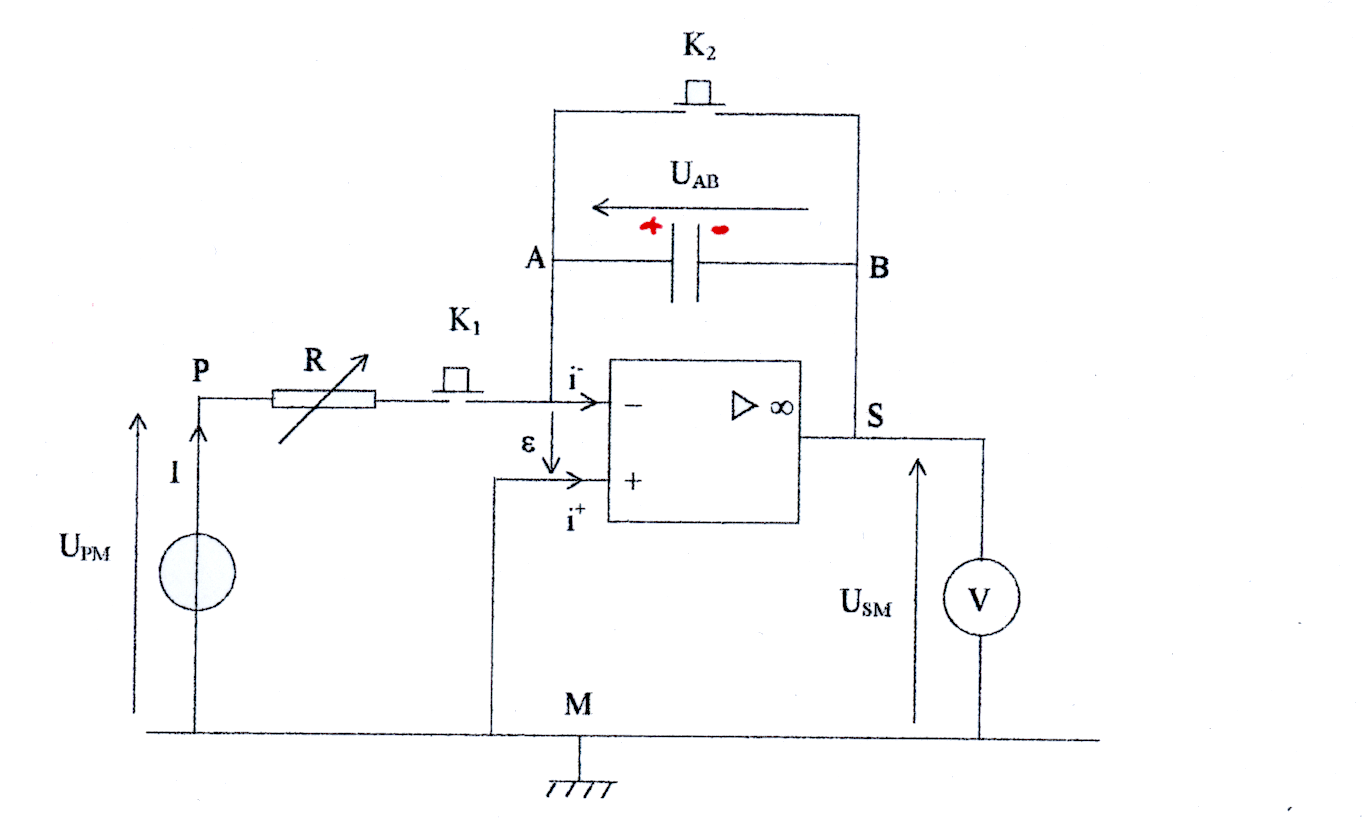
\includegraphics{montage_ao_c.png.eps}
\end{center}

